% Created by tikzDevice version 0.12.3.1 on 2022-04-05 00:21:36
% !TEX encoding = UTF-8 Unicode
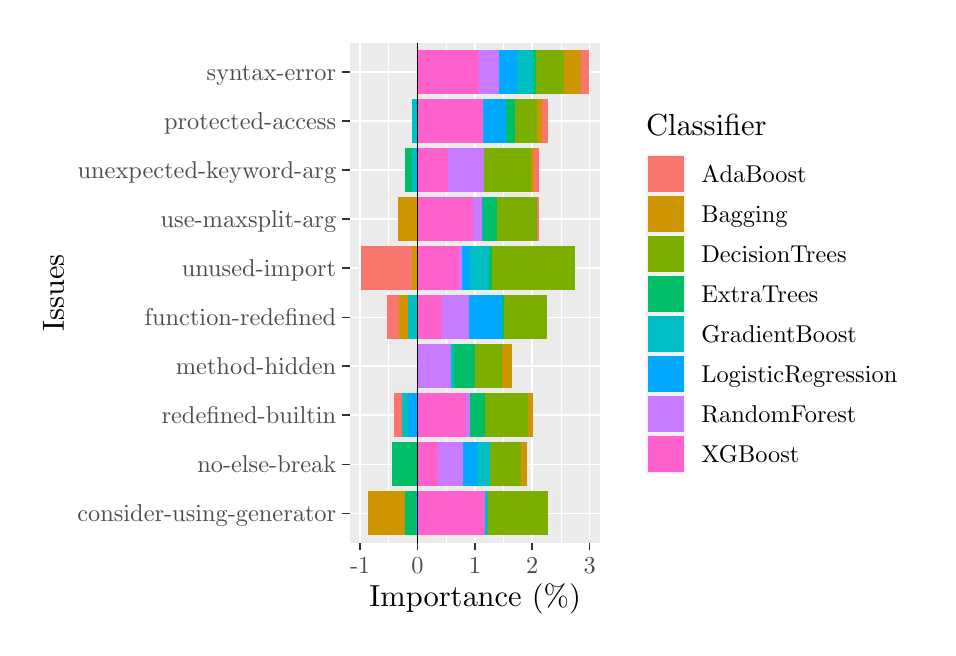
\begin{tikzpicture}[x=1pt,y=1pt]
\definecolor{fillColor}{RGB}{255,255,255}
\path[use as bounding box,fill=fillColor,fill opacity=0.00] (0,0) rectangle (325.21,216.81);
\begin{scope}
\path[clip] (  0.00,  0.00) rectangle (325.21,216.81);
\definecolor{drawColor}{RGB}{255,255,255}
\definecolor{fillColor}{RGB}{255,255,255}

\path[draw=drawColor,line width= 0.6pt,line join=round,line cap=round,fill=fillColor] (  0.00,  0.00) rectangle (325.21,216.81);
\end{scope}
\begin{scope}
\path[clip] (116.44, 30.69) rectangle (206.96,211.31);
\definecolor{fillColor}{gray}{0.92}

\path[fill=fillColor] (116.44, 30.69) rectangle (206.96,211.31);
\definecolor{drawColor}{RGB}{255,255,255}

\path[draw=drawColor,line width= 0.3pt,line join=round] (130.51, 30.69) --
	(130.51,211.31);

\path[draw=drawColor,line width= 0.3pt,line join=round] (151.23, 30.69) --
	(151.23,211.31);

\path[draw=drawColor,line width= 0.3pt,line join=round] (171.96, 30.69) --
	(171.96,211.31);

\path[draw=drawColor,line width= 0.3pt,line join=round] (192.69, 30.69) --
	(192.69,211.31);

\path[draw=drawColor,line width= 0.6pt,line join=round] (116.44, 41.31) --
	(206.96, 41.31);

\path[draw=drawColor,line width= 0.6pt,line join=round] (116.44, 59.02) --
	(206.96, 59.02);

\path[draw=drawColor,line width= 0.6pt,line join=round] (116.44, 76.73) --
	(206.96, 76.73);

\path[draw=drawColor,line width= 0.6pt,line join=round] (116.44, 94.44) --
	(206.96, 94.44);

\path[draw=drawColor,line width= 0.6pt,line join=round] (116.44,112.14) --
	(206.96,112.14);

\path[draw=drawColor,line width= 0.6pt,line join=round] (116.44,129.85) --
	(206.96,129.85);

\path[draw=drawColor,line width= 0.6pt,line join=round] (116.44,147.56) --
	(206.96,147.56);

\path[draw=drawColor,line width= 0.6pt,line join=round] (116.44,165.27) --
	(206.96,165.27);

\path[draw=drawColor,line width= 0.6pt,line join=round] (116.44,182.98) --
	(206.96,182.98);

\path[draw=drawColor,line width= 0.6pt,line join=round] (116.44,200.69) --
	(206.96,200.69);

\path[draw=drawColor,line width= 0.6pt,line join=round] (120.14, 30.69) --
	(120.14,211.31);

\path[draw=drawColor,line width= 0.6pt,line join=round] (140.87, 30.69) --
	(140.87,211.31);

\path[draw=drawColor,line width= 0.6pt,line join=round] (161.60, 30.69) --
	(161.60,211.31);

\path[draw=drawColor,line width= 0.6pt,line join=round] (182.33, 30.69) --
	(182.33,211.31);

\path[draw=drawColor,line width= 0.6pt,line join=round] (203.06, 30.69) --
	(203.06,211.31);
\definecolor{fillColor}{RGB}{248,118,109}

\path[fill=fillColor] (199.95,192.72) rectangle (202.85,208.65);

\path[fill=fillColor] (185.85,175.01) rectangle (187.92,190.95);

\path[fill=fillColor] (182.95,157.30) rectangle (184.61,173.24);

\path[fill=fillColor] (120.56,121.88) rectangle (138.80,137.82);

\path[fill=fillColor] (183.98,139.59) rectangle (184.61,155.53);

\path[fill=fillColor] (129.88,104.18) rectangle (134.24,120.11);

\path[fill=fillColor] (174.86, 86.47) rectangle (174.86,102.40);

\path[fill=fillColor] (132.37, 68.76) rectangle (135.27, 84.70);

\path[fill=fillColor] (180.25, 51.05) rectangle (180.25, 66.99);

\path[fill=fillColor] (122.84, 33.34) rectangle (123.04, 49.28);
\definecolor{fillColor}{RGB}{205,150,0}

\path[fill=fillColor] (193.93,192.72) rectangle (199.95,208.65);

\path[fill=fillColor] (183.98,175.01) rectangle (185.85,190.95);

\path[fill=fillColor] (181.70,157.30) rectangle (182.95,173.24);

\path[fill=fillColor] (138.80,121.88) rectangle (140.87,137.82);

\path[fill=fillColor] (133.82,139.59) rectangle (140.87,155.53);

\path[fill=fillColor] (134.24,104.18) rectangle (137.35,120.11);

\path[fill=fillColor] (171.55, 86.47) rectangle (174.86,102.40);

\path[fill=fillColor] (180.67, 68.76) rectangle (182.74, 84.70);

\path[fill=fillColor] (178.18, 51.05) rectangle (180.25, 66.99);

\path[fill=fillColor] (123.04, 33.34) rectangle (136.31, 49.28);
\definecolor{fillColor}{RGB}{124,174,0}

\path[fill=fillColor] (183.78,192.72) rectangle (193.93,208.65);

\path[fill=fillColor] (176.11,175.01) rectangle (183.98,190.95);

\path[fill=fillColor] (164.91,157.30) rectangle (181.70,173.24);

\path[fill=fillColor] (167.61,121.88) rectangle (197.87,137.82);

\path[fill=fillColor] (169.47,139.59) rectangle (183.98,155.53);

\path[fill=fillColor] (171.96,104.18) rectangle (187.51,120.11);

\path[fill=fillColor] (161.60, 86.47) rectangle (171.55,102.40);

\path[fill=fillColor] (165.33, 68.76) rectangle (180.67, 84.70);

\path[fill=fillColor] (166.99, 51.05) rectangle (178.18, 66.99);

\path[fill=fillColor] (166.37, 33.34) rectangle (188.13, 49.28);
\definecolor{fillColor}{RGB}{0,190,103}

\path[fill=fillColor] (182.53,192.72) rectangle (183.78,208.65);

\path[fill=fillColor] (172.79,175.01) rectangle (176.11,190.95);

\path[fill=fillColor] (136.31,157.30) rectangle (139.00,173.24);

\path[fill=fillColor] (166.78,121.88) rectangle (167.61,137.82);

\path[fill=fillColor] (164.71,139.59) rectangle (169.47,155.53);

\path[fill=fillColor] (171.34,104.18) rectangle (171.96,120.11);

\path[fill=fillColor] (153.93, 86.47) rectangle (161.60,102.40);

\path[fill=fillColor] (159.73, 68.76) rectangle (165.33, 84.70);

\path[fill=fillColor] (131.75, 51.05) rectangle (140.87, 66.99);

\path[fill=fillColor] (136.31, 33.34) rectangle (140.25, 49.28);
\definecolor{fillColor}{RGB}{0,191,196}

\path[fill=fillColor] (176.73,192.72) rectangle (182.53,208.65);

\path[fill=fillColor] (138.80,175.01) rectangle (140.87,190.95);

\path[fill=fillColor] (139.00,157.30) rectangle (140.25,173.24);

\path[fill=fillColor] (159.94,121.88) rectangle (166.78,137.82);

\path[fill=fillColor] (164.71,139.59) rectangle (164.71,155.53);

\path[fill=fillColor] (137.35,104.18) rectangle (140.87,120.11);

\path[fill=fillColor] (152.89, 86.47) rectangle (153.93,102.40);

\path[fill=fillColor] (135.27, 68.76) rectangle (137.35, 84.70);

\path[fill=fillColor] (162.22, 51.05) rectangle (166.99, 66.99);

\path[fill=fillColor] (165.12, 33.34) rectangle (166.37, 49.28);
\definecolor{fillColor}{RGB}{0,169,255}

\path[fill=fillColor] (170.30,192.72) rectangle (176.73,208.65);

\path[fill=fillColor] (164.71,175.01) rectangle (172.79,190.95);

\path[fill=fillColor] (140.25,157.30) rectangle (140.87,173.24);

\path[fill=fillColor] (157.04,121.88) rectangle (159.94,137.82);

\path[fill=fillColor] (164.29,139.59) rectangle (164.71,155.53);

\path[fill=fillColor] (159.53,104.18) rectangle (171.34,120.11);

\path[fill=fillColor] (152.89, 86.47) rectangle (152.89,102.40);

\path[fill=fillColor] (137.35, 68.76) rectangle (140.87, 84.70);

\path[fill=fillColor] (157.24, 51.05) rectangle (162.22, 66.99);

\path[fill=fillColor] (140.25, 33.34) rectangle (140.87, 49.28);
\definecolor{fillColor}{RGB}{199,124,255}

\path[fill=fillColor] (163.05,192.72) rectangle (170.30,208.65);

\path[fill=fillColor] (164.71,175.01) rectangle (164.71,190.95);

\path[fill=fillColor] (152.06,157.30) rectangle (164.91,173.24);

\path[fill=fillColor] (156.00,121.88) rectangle (157.04,137.82);

\path[fill=fillColor] (160.98,139.59) rectangle (164.29,155.53);

\path[fill=fillColor] (149.58,104.18) rectangle (159.53,120.11);

\path[fill=fillColor] (140.87, 86.47) rectangle (152.89,102.40);

\path[fill=fillColor] (158.49, 68.76) rectangle (159.73, 84.70);

\path[fill=fillColor] (148.33, 51.05) rectangle (157.24, 66.99);

\path[fill=fillColor] (165.12, 33.34) rectangle (165.12, 49.28);
\definecolor{fillColor}{RGB}{255,97,204}

\path[fill=fillColor] (140.87,192.72) rectangle (163.05,208.65);

\path[fill=fillColor] (140.87,175.01) rectangle (164.71,190.95);

\path[fill=fillColor] (140.87,157.30) rectangle (152.06,173.24);

\path[fill=fillColor] (140.87,121.88) rectangle (156.00,137.82);

\path[fill=fillColor] (140.87,139.59) rectangle (160.98,155.53);

\path[fill=fillColor] (140.87,104.18) rectangle (149.58,120.11);

\path[fill=fillColor] (140.87, 86.47) rectangle (140.87,102.40);

\path[fill=fillColor] (140.87, 68.76) rectangle (158.49, 84.70);

\path[fill=fillColor] (140.87, 51.05) rectangle (148.33, 66.99);

\path[fill=fillColor] (140.87, 33.34) rectangle (165.12, 49.28);
\definecolor{drawColor}{RGB}{0,0,0}

\path[draw=drawColor,line width= 0.6pt,line join=round] (140.87, 30.69) -- (140.87,211.31);
\end{scope}
\begin{scope}
\path[clip] (  0.00,  0.00) rectangle (325.21,216.81);
\definecolor{drawColor}{gray}{0.30}

\node[text=drawColor,anchor=base east,inner sep=0pt, outer sep=0pt, scale=  0.88] at (111.49, 38.28) {consider-using-generator};

\node[text=drawColor,anchor=base east,inner sep=0pt, outer sep=0pt, scale=  0.88] at (111.49, 55.99) {no-else-break};

\node[text=drawColor,anchor=base east,inner sep=0pt, outer sep=0pt, scale=  0.88] at (111.49, 73.70) {redefined-builtin};

\node[text=drawColor,anchor=base east,inner sep=0pt, outer sep=0pt, scale=  0.88] at (111.49, 91.41) {method-hidden};

\node[text=drawColor,anchor=base east,inner sep=0pt, outer sep=0pt, scale=  0.88] at (111.49,109.11) {function-redefined};

\node[text=drawColor,anchor=base east,inner sep=0pt, outer sep=0pt, scale=  0.88] at (111.49,126.82) {unused-import};

\node[text=drawColor,anchor=base east,inner sep=0pt, outer sep=0pt, scale=  0.88] at (111.49,144.53) {use-maxsplit-arg};

\node[text=drawColor,anchor=base east,inner sep=0pt, outer sep=0pt, scale=  0.88] at (111.49,162.24) {unexpected-keyword-arg};

\node[text=drawColor,anchor=base east,inner sep=0pt, outer sep=0pt, scale=  0.88] at (111.49,179.95) {protected-access};

\node[text=drawColor,anchor=base east,inner sep=0pt, outer sep=0pt, scale=  0.88] at (111.49,197.65) {syntax-error};
\end{scope}
\begin{scope}
\path[clip] (  0.00,  0.00) rectangle (325.21,216.81);
\definecolor{drawColor}{gray}{0.20}

\path[draw=drawColor,line width= 0.6pt,line join=round] (113.69, 41.31) --
	(116.44, 41.31);

\path[draw=drawColor,line width= 0.6pt,line join=round] (113.69, 59.02) --
	(116.44, 59.02);

\path[draw=drawColor,line width= 0.6pt,line join=round] (113.69, 76.73) --
	(116.44, 76.73);

\path[draw=drawColor,line width= 0.6pt,line join=round] (113.69, 94.44) --
	(116.44, 94.44);

\path[draw=drawColor,line width= 0.6pt,line join=round] (113.69,112.14) --
	(116.44,112.14);

\path[draw=drawColor,line width= 0.6pt,line join=round] (113.69,129.85) --
	(116.44,129.85);

\path[draw=drawColor,line width= 0.6pt,line join=round] (113.69,147.56) --
	(116.44,147.56);

\path[draw=drawColor,line width= 0.6pt,line join=round] (113.69,165.27) --
	(116.44,165.27);

\path[draw=drawColor,line width= 0.6pt,line join=round] (113.69,182.98) --
	(116.44,182.98);

\path[draw=drawColor,line width= 0.6pt,line join=round] (113.69,200.69) --
	(116.44,200.69);
\end{scope}
\begin{scope}
\path[clip] (  0.00,  0.00) rectangle (325.21,216.81);
\definecolor{drawColor}{gray}{0.20}

\path[draw=drawColor,line width= 0.6pt,line join=round] (120.14, 27.94) --
	(120.14, 30.69);

\path[draw=drawColor,line width= 0.6pt,line join=round] (140.87, 27.94) --
	(140.87, 30.69);

\path[draw=drawColor,line width= 0.6pt,line join=round] (161.60, 27.94) --
	(161.60, 30.69);

\path[draw=drawColor,line width= 0.6pt,line join=round] (182.33, 27.94) --
	(182.33, 30.69);

\path[draw=drawColor,line width= 0.6pt,line join=round] (203.06, 27.94) --
	(203.06, 30.69);
\end{scope}
\begin{scope}
\path[clip] (  0.00,  0.00) rectangle (325.21,216.81);
\definecolor{drawColor}{gray}{0.30}

\node[text=drawColor,anchor=base,inner sep=0pt, outer sep=0pt, scale=  0.88] at (120.14, 19.68) {-1};

\node[text=drawColor,anchor=base,inner sep=0pt, outer sep=0pt, scale=  0.88] at (140.87, 19.68) {0};

\node[text=drawColor,anchor=base,inner sep=0pt, outer sep=0pt, scale=  0.88] at (161.60, 19.68) {1};

\node[text=drawColor,anchor=base,inner sep=0pt, outer sep=0pt, scale=  0.88] at (182.33, 19.68) {2};

\node[text=drawColor,anchor=base,inner sep=0pt, outer sep=0pt, scale=  0.88] at (203.06, 19.68) {3};
\end{scope}
\begin{scope}
\path[clip] (  0.00,  0.00) rectangle (325.21,216.81);
\definecolor{drawColor}{RGB}{0,0,0}

\node[text=drawColor,anchor=base,inner sep=0pt, outer sep=0pt, scale=  1.10] at (161.70,  7.64) {Importance (\%)};
\end{scope}
\begin{scope}
\path[clip] (  0.00,  0.00) rectangle (325.21,216.81);
\definecolor{drawColor}{RGB}{0,0,0}

\node[text=drawColor,rotate= 90.00,anchor=base,inner sep=0pt, outer sep=0pt, scale=  1.10] at ( 13.08,121.00) {Issues};
\end{scope}
\begin{scope}
\path[clip] (  0.00,  0.00) rectangle (325.21,216.81);
\definecolor{fillColor}{RGB}{255,255,255}

\path[fill=fillColor] (217.96, 50.07) rectangle (319.71,191.92);
\end{scope}
\begin{scope}
\path[clip] (  0.00,  0.00) rectangle (325.21,216.81);
\definecolor{drawColor}{RGB}{0,0,0}

\node[text=drawColor,anchor=base west,inner sep=0pt, outer sep=0pt, scale=  1.10] at (223.46,177.78) {Classifier};
\end{scope}
\begin{scope}
\path[clip] (  0.00,  0.00) rectangle (325.21,216.81);
\definecolor{fillColor}{gray}{0.95}

\path[fill=fillColor] (223.46,156.75) rectangle (237.92,171.21);
\end{scope}
\begin{scope}
\path[clip] (  0.00,  0.00) rectangle (325.21,216.81);
\definecolor{fillColor}{RGB}{248,118,109}

\path[fill=fillColor] (224.17,157.46) rectangle (237.21,170.50);
\end{scope}
\begin{scope}
\path[clip] (  0.00,  0.00) rectangle (325.21,216.81);
\definecolor{fillColor}{gray}{0.95}

\path[fill=fillColor] (223.46,142.30) rectangle (237.92,156.75);
\end{scope}
\begin{scope}
\path[clip] (  0.00,  0.00) rectangle (325.21,216.81);
\definecolor{fillColor}{RGB}{205,150,0}

\path[fill=fillColor] (224.17,143.01) rectangle (237.21,156.04);
\end{scope}
\begin{scope}
\path[clip] (  0.00,  0.00) rectangle (325.21,216.81);
\definecolor{fillColor}{gray}{0.95}

\path[fill=fillColor] (223.46,127.84) rectangle (237.92,142.30);
\end{scope}
\begin{scope}
\path[clip] (  0.00,  0.00) rectangle (325.21,216.81);
\definecolor{fillColor}{RGB}{124,174,0}

\path[fill=fillColor] (224.17,128.56) rectangle (237.21,141.59);
\end{scope}
\begin{scope}
\path[clip] (  0.00,  0.00) rectangle (325.21,216.81);
\definecolor{fillColor}{gray}{0.95}

\path[fill=fillColor] (223.46,113.39) rectangle (237.92,127.84);
\end{scope}
\begin{scope}
\path[clip] (  0.00,  0.00) rectangle (325.21,216.81);
\definecolor{fillColor}{RGB}{0,190,103}

\path[fill=fillColor] (224.17,114.10) rectangle (237.21,127.13);
\end{scope}
\begin{scope}
\path[clip] (  0.00,  0.00) rectangle (325.21,216.81);
\definecolor{fillColor}{gray}{0.95}

\path[fill=fillColor] (223.46, 98.94) rectangle (237.92,113.39);
\end{scope}
\begin{scope}
\path[clip] (  0.00,  0.00) rectangle (325.21,216.81);
\definecolor{fillColor}{RGB}{0,191,196}

\path[fill=fillColor] (224.17, 99.65) rectangle (237.21,112.68);
\end{scope}
\begin{scope}
\path[clip] (  0.00,  0.00) rectangle (325.21,216.81);
\definecolor{fillColor}{gray}{0.95}

\path[fill=fillColor] (223.46, 84.48) rectangle (237.92, 98.94);
\end{scope}
\begin{scope}
\path[clip] (  0.00,  0.00) rectangle (325.21,216.81);
\definecolor{fillColor}{RGB}{0,169,255}

\path[fill=fillColor] (224.17, 85.19) rectangle (237.21, 98.23);
\end{scope}
\begin{scope}
\path[clip] (  0.00,  0.00) rectangle (325.21,216.81);
\definecolor{fillColor}{gray}{0.95}

\path[fill=fillColor] (223.46, 70.03) rectangle (237.92, 84.48);
\end{scope}
\begin{scope}
\path[clip] (  0.00,  0.00) rectangle (325.21,216.81);
\definecolor{fillColor}{RGB}{199,124,255}

\path[fill=fillColor] (224.17, 70.74) rectangle (237.21, 83.77);
\end{scope}
\begin{scope}
\path[clip] (  0.00,  0.00) rectangle (325.21,216.81);
\definecolor{fillColor}{gray}{0.95}

\path[fill=fillColor] (223.46, 55.57) rectangle (237.92, 70.03);
\end{scope}
\begin{scope}
\path[clip] (  0.00,  0.00) rectangle (325.21,216.81);
\definecolor{fillColor}{RGB}{255,97,204}

\path[fill=fillColor] (224.17, 56.29) rectangle (237.21, 69.32);
\end{scope}
\begin{scope}
\path[clip] (  0.00,  0.00) rectangle (325.21,216.81);
\definecolor{drawColor}{RGB}{0,0,0}

\node[text=drawColor,anchor=base west,inner sep=0pt, outer sep=0pt, scale=  0.88] at (243.42,160.95) {AdaBoost};
\end{scope}
\begin{scope}
\path[clip] (  0.00,  0.00) rectangle (325.21,216.81);
\definecolor{drawColor}{RGB}{0,0,0}

\node[text=drawColor,anchor=base west,inner sep=0pt, outer sep=0pt, scale=  0.88] at (243.42,146.50) {Bagging};
\end{scope}
\begin{scope}
\path[clip] (  0.00,  0.00) rectangle (325.21,216.81);
\definecolor{drawColor}{RGB}{0,0,0}

\node[text=drawColor,anchor=base west,inner sep=0pt, outer sep=0pt, scale=  0.88] at (243.42,132.04) {DecisionTrees};
\end{scope}
\begin{scope}
\path[clip] (  0.00,  0.00) rectangle (325.21,216.81);
\definecolor{drawColor}{RGB}{0,0,0}

\node[text=drawColor,anchor=base west,inner sep=0pt, outer sep=0pt, scale=  0.88] at (243.42,117.59) {ExtraTrees};
\end{scope}
\begin{scope}
\path[clip] (  0.00,  0.00) rectangle (325.21,216.81);
\definecolor{drawColor}{RGB}{0,0,0}

\node[text=drawColor,anchor=base west,inner sep=0pt, outer sep=0pt, scale=  0.88] at (243.42,103.13) {GradientBoost};
\end{scope}
\begin{scope}
\path[clip] (  0.00,  0.00) rectangle (325.21,216.81);
\definecolor{drawColor}{RGB}{0,0,0}

\node[text=drawColor,anchor=base west,inner sep=0pt, outer sep=0pt, scale=  0.88] at (243.42, 88.68) {LogisticRegression};
\end{scope}
\begin{scope}
\path[clip] (  0.00,  0.00) rectangle (325.21,216.81);
\definecolor{drawColor}{RGB}{0,0,0}

\node[text=drawColor,anchor=base west,inner sep=0pt, outer sep=0pt, scale=  0.88] at (243.42, 74.23) {RandomForest};
\end{scope}
\begin{scope}
\path[clip] (  0.00,  0.00) rectangle (325.21,216.81);
\definecolor{drawColor}{RGB}{0,0,0}

\node[text=drawColor,anchor=base west,inner sep=0pt, outer sep=0pt, scale=  0.88] at (243.42, 59.77) {XGBoost};
\end{scope}
\end{tikzpicture}
